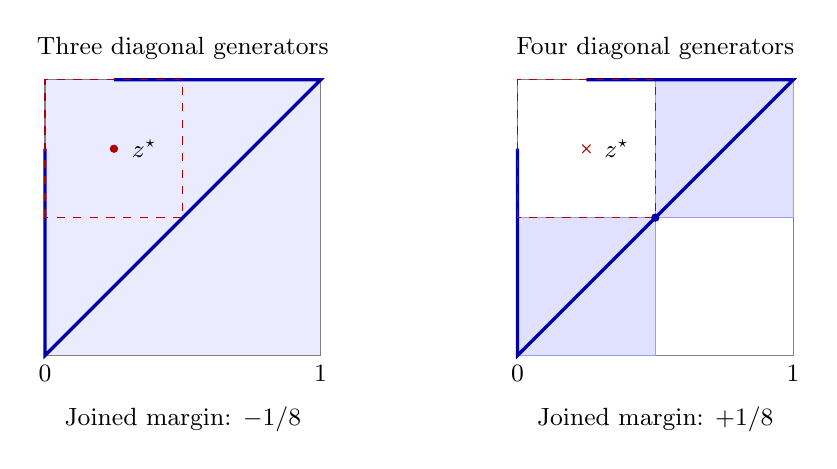
\begin{tikzpicture}[x=3.5cm,y=3.5cm,font=\small]
\begin{scope}
\fill[blue!8] (0,0) rectangle (1,1);
\draw[gray] (0,0) rectangle (1,1);
\draw[very thick,blue!65!black] (0,.75)--(0,0)--(1,1)--(.25,1);
\draw[red!70!black,dashed] (0,.5) rectangle (.5,1);
\fill[red!70!black] (.25,.75) circle (1.5pt);
\node[right] at (.28,.75) {$z^\star$};
\node[below] at (0,0) {$0$};\node[below] at (1,0) {$1$};
\node[above] at (.5,1.04) {Three diagonal generators};
\node[below] at (.5,-.15) {Joined margin: $-1/8$};
\end{scope}
\begin{scope}[xshift=6.0cm]
\fill[blue!12] (0,0) rectangle (.5,.5);
\fill[blue!12] (.5,.5) rectangle (1,1);
\draw[gray] (0,0) rectangle (1,1);
\draw[blue!40] (0,0) rectangle (.5,.5);
\draw[blue!40] (.5,.5) rectangle (1,1);
\draw[very thick,blue!65!black] (0,.75)--(0,0)--(1,1)--(.25,1);
\draw[red!70!black,dashed] (0,.5) rectangle (.5,1);
\draw[red!70!black] (.235,.735)--(.265,.765) (.235,.765)--(.265,.735);
\node[right] at (.28,.75) {$z^\star$};
\fill[blue!65!black] (.5,.5) circle (1.5pt);
\node[below] at (0,0) {$0$};\node[below] at (1,0) {$1$};
\node[above] at (.5,1.04) {Four diagonal generators};
\node[below] at (.5,-.15) {Joined margin: $+1/8$};
\end{scope}
\end{tikzpicture}
